\chapter{Real-Robot Experiments}
\label{chap:real_robot}

This chapter presents the hardware deployment and real-world validation of the memory-attention-enhanced parkour policy described in Chapters~\ref{chap:proposed_method}--\ref{chap:training}. While the simulation experiments in Chapter~\ref{chap:experimental_results} demonstrated the qualitative behaviors enabled by the attention and memory modules, the ultimate test of any sim-to-real pipeline is whether the learned policy transfers to physical terrain without fine-tuning. We deploy the policy on a Unitree G1 humanoid robot and evaluate it across four terrain types: stairs, slopes, a raised platform, and randomly placed large rocks. The results show that the policy produces natural, terrain-adaptive locomotion in the real world, with the attention module enabling proactive terrain awareness and the memory module preserving context when visual information becomes temporarily unavailable.

The chapter is organized as follows. Section~\ref{sec:system_setup} describes the hardware setup and sim-to-real transfer protocol. Section~\ref{sec:terrain_config} details the terrain configurations. Section~\ref{sec:real_results} presents the experimental results for each terrain scenario. Section~\ref{sec:real_discussion} discusses the key findings, and Section~\ref{sec:real_limitations} discusses limitations and lessons learned.

%% ============================================================
\section{System Setup and Sim-to-Real Transfer}
\label{sec:system_setup}
%% ============================================================

\subsection{Hardware Platform}
\label{sec:hardware_platform}

The robot used in all experiments is the Unitree G1 humanoid robot with 29 degrees of freedom (G1-29Dof-TorsoBase configuration). The robot is approximately 1.3\,m tall and weighs approximately 35\,kg including the battery.

\paragraph{Computing architecture.}
Rather than deploying the policy on an onboard computer, the policy inference is performed on an external laptop connected to the robot via an Ethernet cable. The laptop receives sensor data from the robot and sends joint position commands back at 50\,Hz. While this setup introduces a communication dependency (discussed in Section~\ref{sec:real_limitations}), it simplifies the deployment pipeline and provides sufficient computational resources for real-time inference.

\paragraph{Depth perception.}
An Intel RealSense D435i depth camera is mounted on the robot's head (torso link), pitched downward at 47.5$^\circ$ with no yaw or roll offset. The camera provides depth images at $480 \times 270$ resolution and 60\,FPS. The depth camera runs in a separate process and communicates with the main control loop via shared memory, ensuring that the camera's operation does not interfere with the policy inference timing. The RealSense D435i has a vertical field of view (VFOV) of 58.0$^\circ$, which covers a sufficiently wide area in front of and below the robot for terrain perception.

\paragraph{Control loop.}
The main control loop runs at 50\,Hz (20\,ms period), consistent with the simulation training frequency. Each control cycle executes the full observe--infer--act pipeline: (1)~read proprioceptive observations (IMU angular velocity, projected gravity, joint positions and velocities, previous actions, velocity commands) and the latest depth image from the shared memory buffer; (2)~run the ONNX-exported policy network to compute the action; (3)~send the resulting joint position targets to the robot's low-level motor controller.

\subsection{Depth Image Processing Pipeline}
\label{sec:depth_pipeline}

The depth image undergoes a multi-step preprocessing pipeline that mirrors the simulation's camera noise pipeline, ensuring that the real-world input distribution matches what the policy was trained on:

\begin{enumerate}
    \item \textbf{Downsampling.} The raw $480 \times 270$ depth image is downsampled to $64 \times 36$ by sampling the center pixel of each block, matching the simulation camera's ray-caster resolution.
    \item \textbf{Cropping.} The top 18 rows and the left and right 16 columns are removed, yielding a $32 \times 18$ depth image. This cropping removes the sky region and peripheral areas that are less relevant for locomotion.
    \item \textbf{Gaussian blur.} A $3 \times 3$ Gaussian kernel with $\sigma = 1$ is applied for smoothing.
    \item \textbf{Depth normalization.} Depth values are clipped to $[0, 2.5]$\,m and linearly mapped to $[0, 1]$.
    \item \textbf{Temporal stacking with frame subsampling.} The policy receives a stack of 8 depth frames subsampled from a 37-frame history buffer at intervals of 5 frames, providing an effective temporal horizon of approximately 3.6\,s ($37 \times 0.02$\,s). This temporal stacking is the mechanism that provides the policy with longer-range depth information, as discussed in Section~\ref{sec:attention_memory_synergy}.
\end{enumerate}

\subsection{Actuator Model}
\label{sec:actuator_model}

The sim-to-real transfer for the actuator layer follows the BeyondMimic actuator modeling approach. Each joint is modeled as a delayed PD actuator with motor-specific armature values derived from the physical motor parameters (Unitree A1-7520 and A1-5020 motor series). The stiffness and damping gains are computed from the armature values using a natural frequency of 10\,Hz and a damping ratio of 2.0:
\begin{equation}
    k_p = b \cdot \omega_n^2, \quad k_d = 2\zeta \, b \cdot \omega_n
    \label{eq:actuator_gains}
\end{equation}
where $b$ is the armature, $\omega_n = 10 \times 2\pi$\,rad/s is the natural frequency, and $\zeta = 2.0$ is the damping ratio. An actuator delay of 0--2 timesteps (0--40\,ms) is applied during training to account for communication and computation latency. The resulting PD gains are used directly on the real robot's low-level joint position controller without any gain tuning.

Table~\ref{tab:actuator_params} summarizes the actuator parameters for the major joint groups.

\begin{table}[t]
\centering
\caption{Actuator parameters for the G1-29Dof-TorsoBase configuration. Stiffness and damping are computed from Eq.~\ref{eq:actuator_gains}.}
\label{tab:actuator_params}
\footnotesize
\begin{tabular}{@{}p{2.5cm}p{2.8cm}ccccc@{}}
\toprule
\textbf{Joint Group} & \textbf{Motor} & \textbf{Armature} & $\boldsymbol{k_p}$ (N\,m/rad) & $\boldsymbol{k_d}$ (N\,m\,s/rad) & \textbf{Effort Limit} (N\,m) \\
\midrule
Hip pitch / yaw   & A1-7520 (14\,A) & 0.0102 & 40.2  & 2.56  & 88  \\
Hip roll / knee   & A1-7520 (22\,A) & 0.0251 & 99.1  & 6.31  & 139 \\
Ankle pitch/roll  & A1-5020 ($\times$2) & 0.0072 & 28.5  & 1.82  & 50  \\
Waist roll/pitch  & A1-5020 ($\times$2) & 0.0072 & 28.5  & 1.82  & 50  \\
Waist yaw         & A1-7520 (14\,A) & 0.0102 & 40.2  & 2.56  & 88  \\
Arms              & A1-5020 / 4010  & varies & varies & varies & 5--25 \\
\bottomrule
\end{tabular}
\end{table}

\subsection{Sim-to-Real Transfer Protocol}
\label{sec:sim2real_protocol}

The policy is trained entirely in simulation using the Isaac Lab framework described in Chapter~\ref{chap:training} and deployed to the real robot without any fine-tuning on real-world data. The sim-to-real gap is bridged through the following techniques:

\begin{itemize}
    \item \textbf{Domain randomization:} As described in Chapter~\ref{chap:proposed_method}, the training environment randomizes friction coefficients, mass distributions, sensor noise (additive uniform noise on proprioceptive observations), depth image noise (Gaussian blur, depth artifacts, random Gaussian noise), and actuator delays (0--2 timesteps) to cover the range of real-world variability.
    \item \textbf{Depth image preprocessing:} The real depth images undergo the same preprocessing pipeline as in simulation (Section~\ref{sec:depth_pipeline}), including downsampling, cropping, Gaussian blur, depth normalization, and temporal stacking with frame subsampling.
    \item \textbf{Actuator model:} The delayed PD actuator model in simulation (Section~\ref{sec:actuator_model}) is designed to match the real actuator dynamics. The same PD gains are used on the real robot without any gain tuning.
    \item \textbf{ONNX export:} The trained PyTorch policy is exported to ONNX format and executed via the ONNX Runtime on the laptop, ensuring deterministic and efficient inference.
\end{itemize}

\subsection{Safety Considerations}
\label{sec:safety}

During testing, a safety harness was attached to the robot's shoulders to prevent damage from falls. The harness was slack at all times and did not apply any external force to the robot during normal operation; it served solely as a safety net in case of a fall. However, occasional inadvertent tension in the harness caused the robot to produce unnecessary balance corrections, which are visible in the supplementary video. This is a limitation of the experimental setup rather than the policy itself.

An important motivation for the safety harness was a communication reliability issue encountered during early testing: the Ethernet cable connector was prone to loosening, causing intermittent communication loss between the laptop and the robot. When communication is lost, the robot continues executing the last received command, which can lead to a fall. During early testing, one such fall resulted in the robot kicking the operator, causing injury. To prevent similar incidents, all subsequent experiments were conducted with the safety harness.

%% ============================================================
\section{Terrain Configurations}
\label{sec:terrain_config}
%% ============================================================

Four terrain types are constructed for the real-robot experiments, each targeting a different aspect of parkour locomotion. Figure~\ref{fig:terrain_overview} shows the overall experimental setup. The specifications of each terrain module are summarized in Table~\ref{tab:terrain_specs}.

\begin{figure}[t]
    \centering
    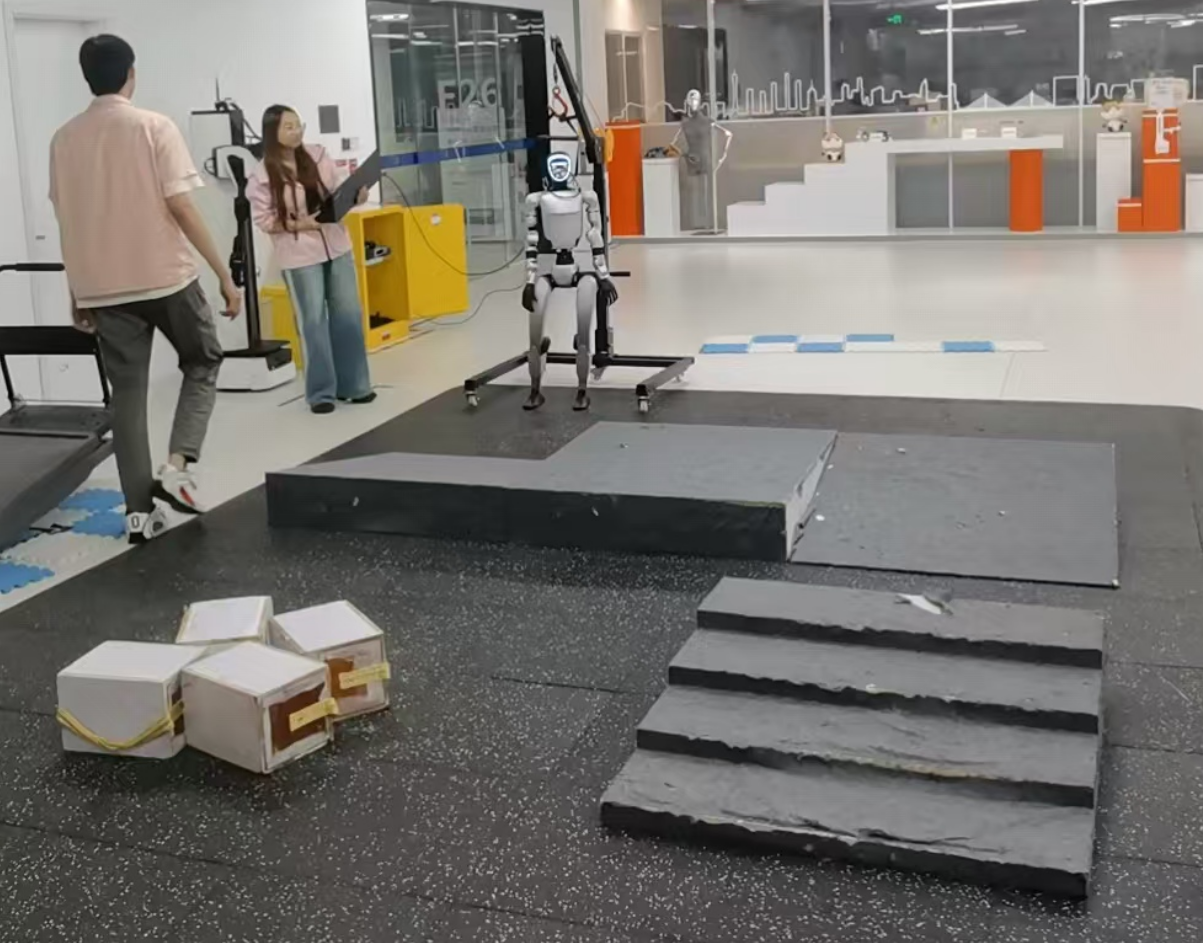
\includegraphics[width=\textwidth]{figures/ch7_terrain_overview.png}
    \caption{Overview of the real-robot experiment terrain setup. The four terrain types are: (a)~stairs connected to a slope, (b)~a second slope from the opposite direction, (c)~randomly placed large rocks, and (d)~a raised platform.}
    \label{fig:terrain_overview}
\end{figure}

\begin{table}[t]
\centering
\caption{Specifications of the terrain modules used in the real-robot experiments.}
\label{tab:terrain_specs}
\footnotesize
\begin{tabular}{@{}p{2.5cm}p{2.5cm}p{7.5cm}@{}}
\toprule
\textbf{Terrain} & \textbf{Footprint} & \textbf{Key Parameters} \\
\midrule
Stairs           & 1\,m $\times$ 1\,m & Total height 20\,cm, 4 steps; each step: width 1\,m, depth 25\,cm, height 5\,cm \\
Slope ($\times$2) & 1\,m $\times$ 1\,m & Height 20\,cm, slope angle $\arctan(0.2) \approx 11.3^\circ$ \\
Raised platform  & 1\,m $\times$ 1\,m & Height 20\,cm \\
Random rocks ($\times$4) & Each 30\,cm $\times$ 22\,cm $\times$ 20\,cm & Randomly placed on flat ground \\
\bottomrule
\end{tabular}
\end{table}

The stair and slope modules are arranged in sequence (stairs $\to$ slope) to test the policy's ability to transition between terrain types. The two slope modules are placed in different orientations to test directional robustness. The raised platform is tested from both approach directions (ascending and descending). The four rock blocks are placed at arbitrary positions and orientations on flat ground to create an unstructured stepping challenge.

All terrain modules share a common height of 20\,cm, which is comparable to the robot's foot length and represents a significant obstacle relative to the robot's leg length. The stair steps (5\,cm each) are intentionally low to test whether the policy can choose efficient multi-step climbing strategies rather than stepping on each individual tread.

%% ============================================================
\section{Experiment Results}
\label{sec:real_results}
%% ============================================================

Each terrain scenario was tested 2--3 times. The initial attempts had lower success rates due to infrastructure issues rather than policy failures: (1)~the Ethernet cable connector loosening during motion, causing communication loss; (2)~the laptop entering power-saving mode during long test sessions, reducing inference speed below the 50\,Hz requirement; and (3)~overly aggressive velocity commands sent via the wireless controller (maximum speed setting), causing excessively large motion amplitudes. Once these infrastructure and operational issues were resolved, the policy consistently produced stable locomotion across all terrain types at a walking speed of approximately 1\,m/s.

\subsection{Stairs Connected to Slope (First Run)}
\label{sec:stair_slope_first}

The first test scenario consists of the stair module connected to a slope module, requiring the robot to climb stairs, transition onto a slope, and descend from the slope to flat ground.

\paragraph{Stair climbing.}
Because each stair step is only 5\,cm high, the robot chooses to take two steps at a time, effectively treating the stairs as 10\,cm steps. This behavior emerges naturally from the policy's terrain-adaptive stepping strategy: the attention module perceives the low step height and determines that a single-step-per-stair gait would be unnecessarily cautious, while the energy penalty reward ($r_{\mathrm{energy}}$, weight $-5 \times 10^{-5}$, defined as the squared sum of torque $\times$ velocity normalized by stiffness) further discourages over-cautious stepping.

\paragraph{Attention-driven step placement at stair end.}
As the robot approaches the top of the stairs, the attention module detects the height difference at the stair-slope boundary. Rather than stepping onto the slope directly from the second-to-last step, the robot places its final step on the last stair tread, ensuring a stable foothold before transitioning to the slope (Figure~\ref{fig:stair_attention_last_step}). This behavior demonstrates that the attention module is not merely reacting to the current depth image but is integrating terrain context to plan the next foothold.

\begin{figure}[t]
    \centering
    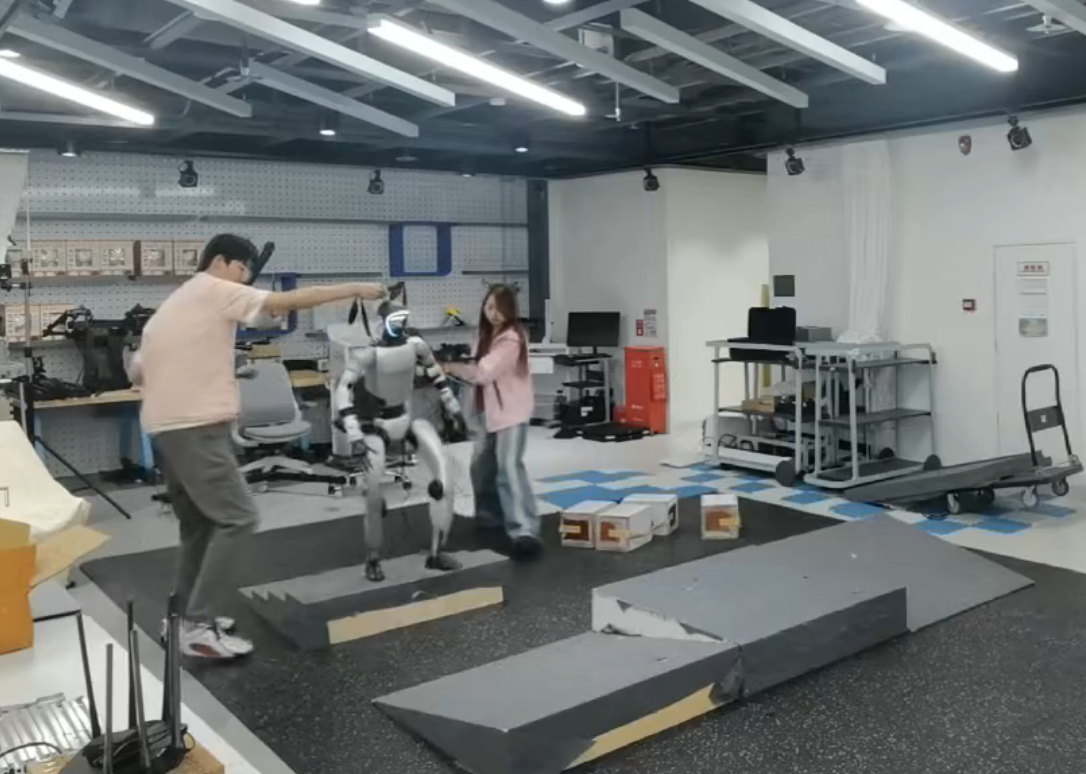
\includegraphics[width=0.9\textwidth]{figures/ch7_stair_attention_last_step.png}
    \caption{The robot climbing stairs connected to a slope. Through the attention mechanism, the robot detects the height difference at the stair end and chooses to place its final step on the last stair tread rather than stepping directly onto the slope, ensuring a stable foothold before the terrain transition.}
    \label{fig:stair_attention_last_step}
\end{figure}

\paragraph{Slope ascent.}
Upon reaching the slope, the depth camera provides visual input indicating the upward incline ahead. The robot responds by lifting its swing foot higher and shifting its center of gravity toward the mid-rear of the support polygon. Placing the center of gravity too far forward would result in insufficient shock absorption at foot landing, causing impact instability. The learned policy naturally adopts this conservative posture, which is consistent with the behavior observed in simulation on pyramid slope terrains (Chapter~\ref{chap:experimental_results}).

\paragraph{Slope descent with attention to edge.}
At the top of the slope, the attention module focuses on the sharp edge where the slope meets the flat ground. To avoid tripping on this edge, the robot adopts a conservative high-step gait for the final step off the slope, lifting the swing foot well above the edge before landing on flat ground (Figure~\ref{fig:slope_attention_edge}). This is another instance where the attention module identifies a specific geometric feature (the slope edge) and the policy adjusts its gait accordingly.

\begin{figure}[t]
    \centering
    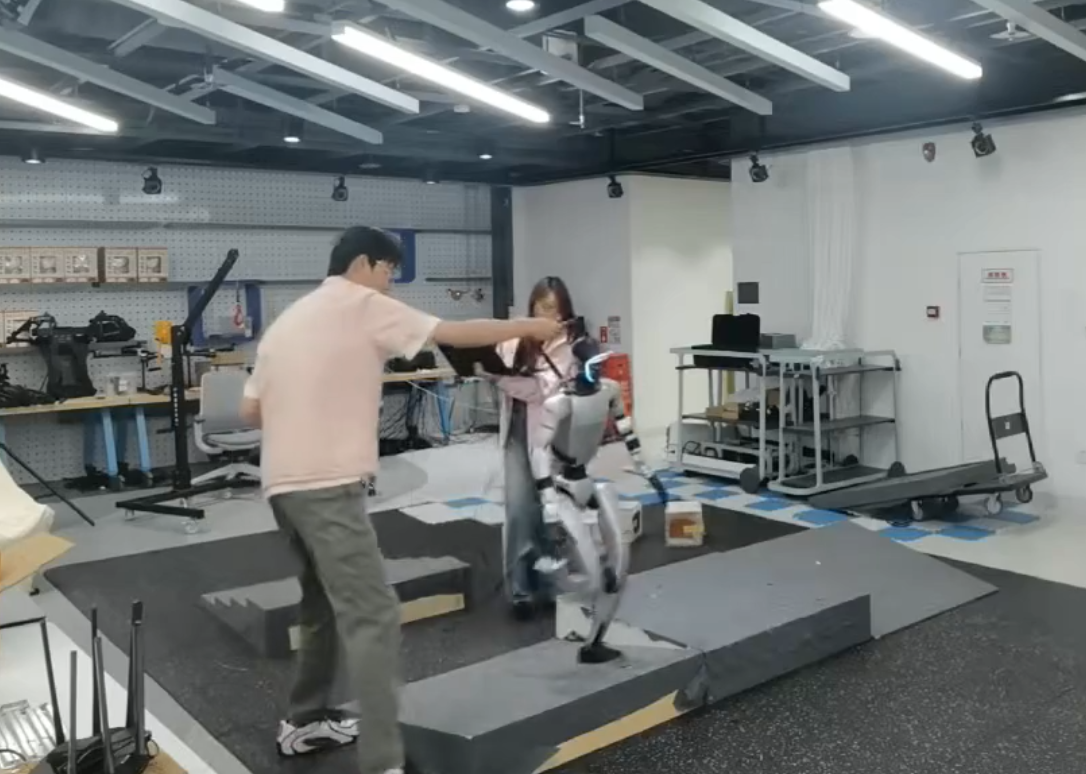
\includegraphics[width=0.9\textwidth]{figures/ch7_slope_attention_edge.png}
    \caption{The robot descending from the slope. The attention module focuses on the sharp edge at the slope top, and the robot adopts a conservative high-step gait to avoid tripping on the edge.}
    \label{fig:slope_attention_edge}
\end{figure}

\subsection{Slope from Opposite Direction}
\label{sec:slope_opposite}

After completing the stair-slope sequence, the robot approaches the second slope module from the opposite direction. The policy produces the same adaptive behaviors---higher foot lift on the slope, rear-shifted center of gravity, and cautious edge descent---demonstrating that the terrain-adaptive strategy is direction-invariant and robust to approach angle.

\subsection{Random Large Rocks}
\label{sec:random_rocks}

The most challenging scenario involves four large rock blocks (each 30\,cm $\times$ 22\,cm $\times$ 20\,cm) placed at arbitrary positions and orientations on flat ground. This terrain tests the combined effect of the attention and memory modules, as the robot must identify stable footholds among the rocks and retain terrain context when visual information becomes occluded.

\paragraph{Step 1: Attention identifies a flat foothold between rocks.}
The attention module identifies a patch of flat ground between two rocks that can serve as a stable foothold. The robot shifts its center of gravity toward this flat region and steps onto it, avoiding the surrounding rocks (Figure~\ref{fig:rocks_attention_memory}, top).

\paragraph{Step 2: Memory preserves terrain context under occlusion.}
After stepping onto the flat ground between the rocks, the depth camera's field of view no longer covers the area directly beneath the robot's feet---the rocks occlude the downward view. However, the memory module retains the information that there are rocks near the feet, and the robot lifts its swing foot high to avoid tripping on the rocks at foot level. This is a clear demonstration of the memory module's value: without memory, the robot would have no knowledge of the rocks beneath it once they leave the camera's field of view, and would likely trip. With memory, the robot proactively lifts its foot and steps securely onto the surface of a rock (Figure~\ref{fig:rocks_attention_memory}, bottom). The synergy between attention and memory is critical here: attention first identifies the flat ground as a stepping target, and memory then preserves the context about nearby rocks even after they leave the camera's view.

\begin{figure}[t]
    \centering
    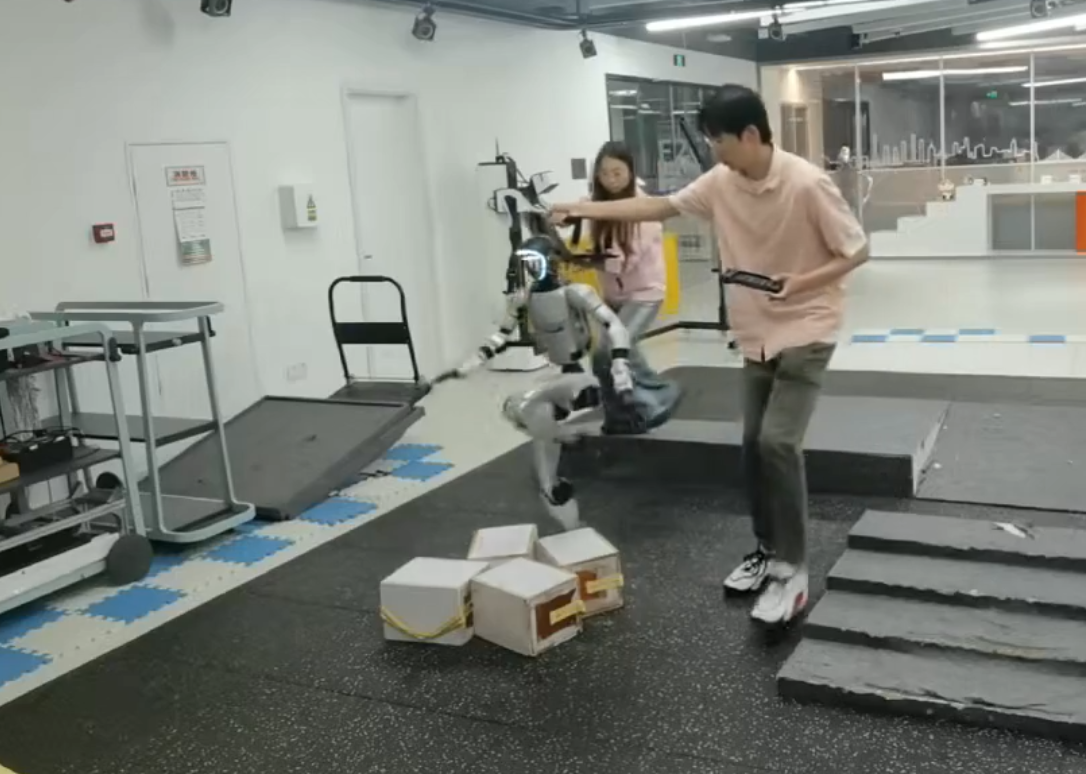
\includegraphics[width=0.9\textwidth]{figures/ch7_rocks_attention_memory.png}
    \caption{The robot navigating randomly placed large rocks. \textbf{Top:} The attention module identifies a flat patch of ground between the rocks and the robot steps onto it. \textbf{Bottom:} After the depth camera can no longer see the area near the feet (rocks occlude the downward view), the memory module retains the terrain context and the robot lifts its swing foot high to avoid tripping, stepping securely onto the rock surface.}
    \label{fig:rocks_attention_memory}
\end{figure}

\paragraph{Step 3: Attention selects the next rock foothold.}
From the top of the first rock, the attention module identifies the next rock's surface as a viable foothold. The robot steps across and lands precisely on the target rock (Figure~\ref{fig:rocks_attention_next_rock}).

\begin{figure}[t]
    \centering
    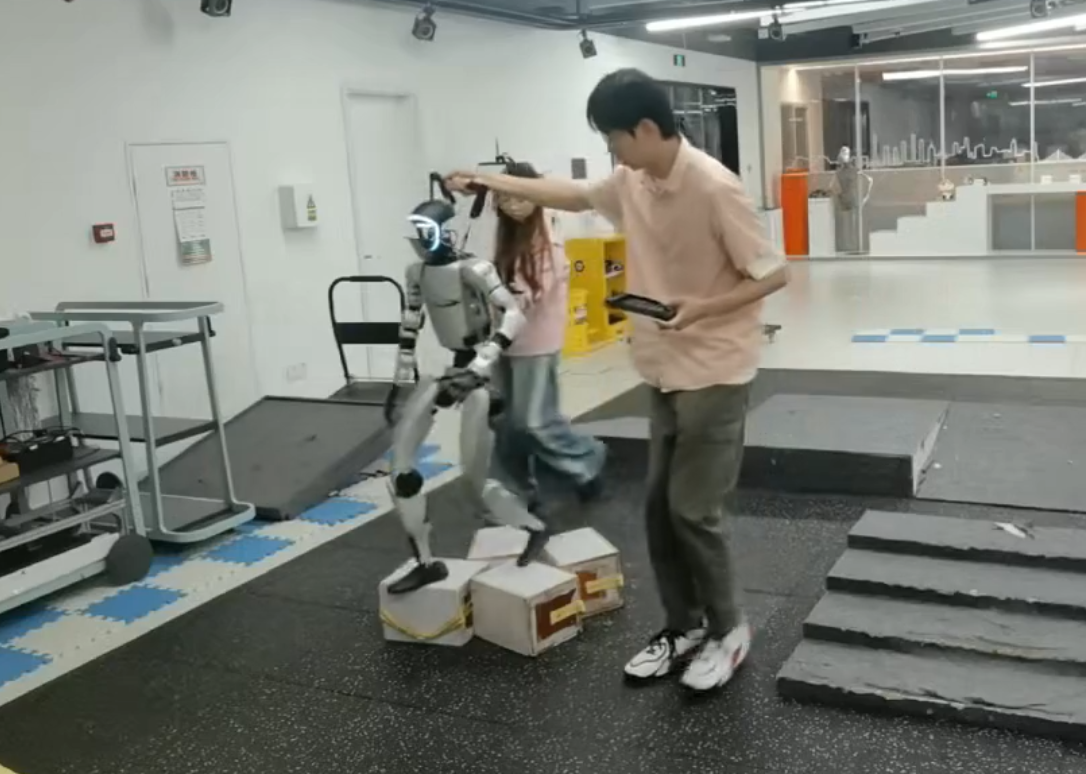
\includegraphics[width=0.9\textwidth]{figures/ch7_rocks_attention_next_rock.png}
    \caption{The robot stepping from one rock to the next. The attention module identifies the next rock's surface as a viable foothold, and the robot lands precisely on the target.}
    \label{fig:rocks_attention_next_rock}
\end{figure}

\paragraph{Step 4: Final step to flat ground.}
After traversing the rocks, the robot steps naturally onto the flat ground between the rocks and lands smoothly (Figure~\ref{fig:rocks_flat_ground}).

\begin{figure}[t]
    \centering
    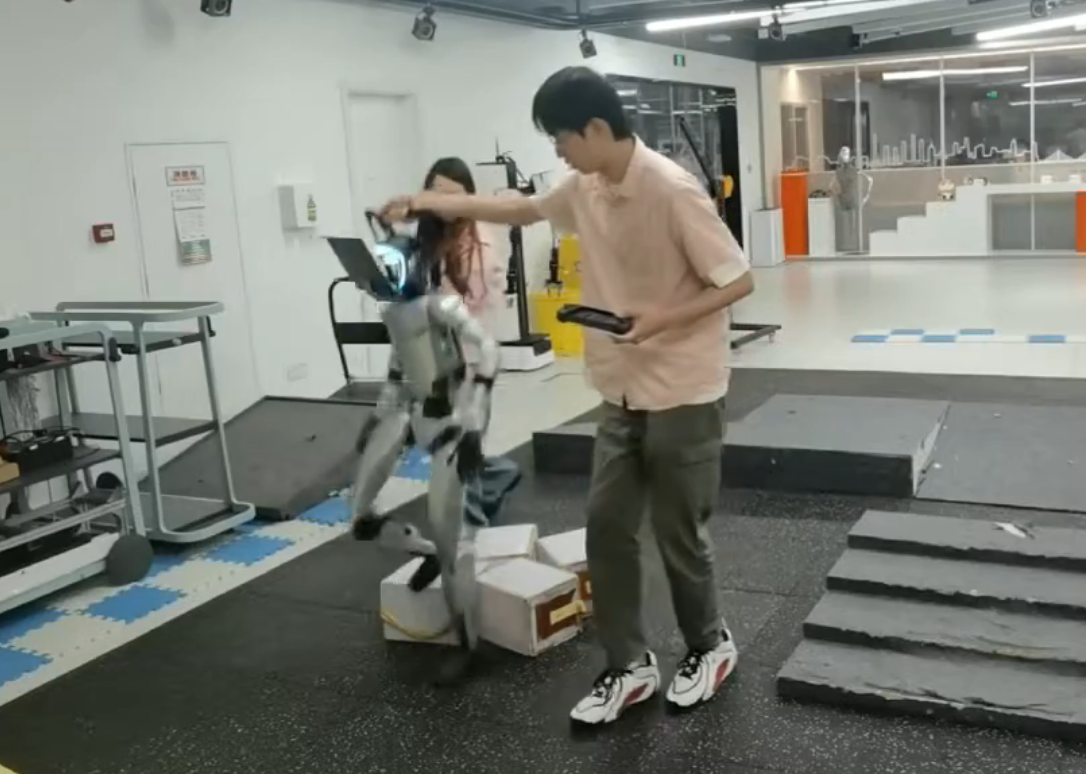
\includegraphics[width=0.9\textwidth]{figures/ch7_rocks_flat_ground.png}
    \caption{The robot's final step from the rocks onto flat ground, landing smoothly.}
    \label{fig:rocks_flat_ground}
\end{figure}

\subsection{Raised Platform}
\label{sec:raised_platform}

The robot is tested on the raised platform (1\,m $\times$ 1\,m, height 20\,cm) from two approach directions: ascending onto the platform and descending from the platform. In both cases, the robot produces natural walking motion without any issues, stepping onto and off the platform with appropriate foot height and body posture.

\subsection{Stairs Connected to Slope (Second Run --- Robustness Verification)}
\label{sec:stair_slope_second}

The stair-slope scenario is repeated to verify the robustness of the policy. In this second run, the robot exhibits a slightly different but equally valid strategy:

\paragraph{Alternative stair strategy.}
Unlike the first run where the robot stepped onto the last stair tread, in this run the robot does not step onto the last step. Instead, it lifts its swing foot over the highest remaining step and lands directly on flat ground beyond the stairs (Figure~\ref{fig:stair_step_over}). This demonstrates that the policy does not follow a fixed behavioral script but makes context-dependent decisions: the attention module perceives the terrain layout, the memory module retains the stair context, and the temporal-subsampled depth image stack provides a longer temporal horizon of depth information. Combined with the energy penalty reward that discourages unnecessary steps, the policy chooses the most efficient action---stepping over the last stair rather than stepping onto it.

\begin{figure}[t]
    \centering
    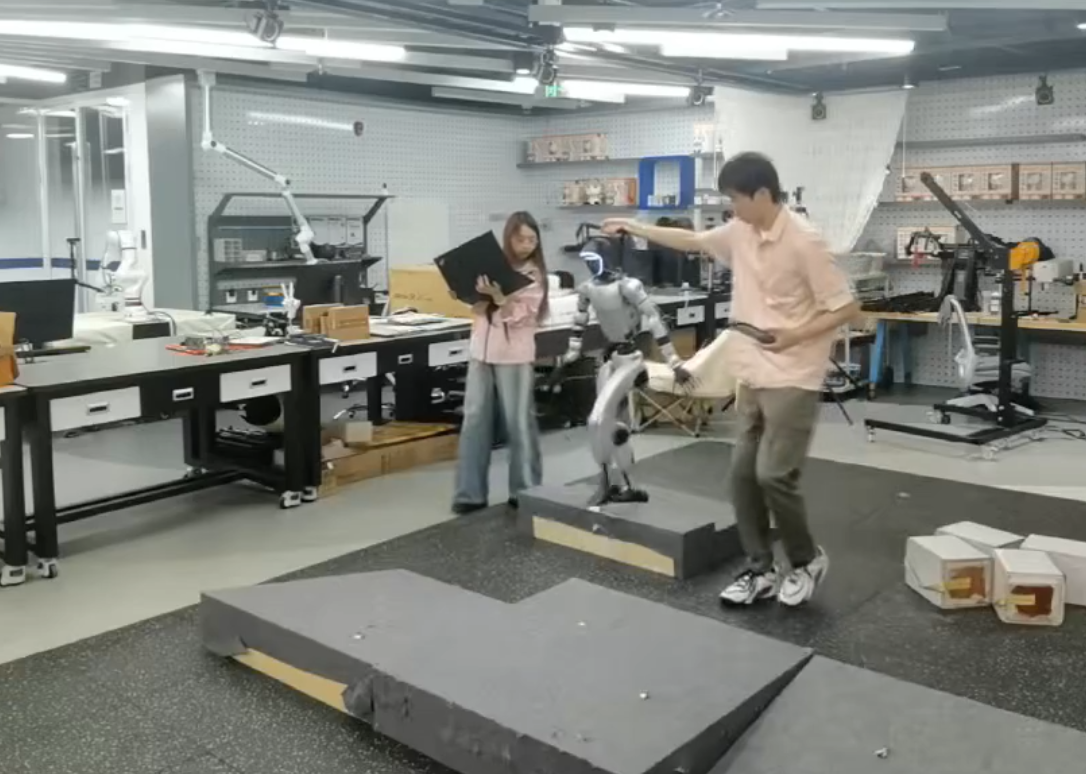
\includegraphics[width=0.9\textwidth]{figures/ch7_stair_step_over.png}
    \caption{The second run on the stair-slope terrain. Unlike the first run, the robot does not step onto the last stair tread but instead lifts its swing foot over the highest step and lands directly on flat ground, demonstrating energy-efficient and context-dependent decision making.}
    \label{fig:stair_step_over}
\end{figure}

\paragraph{Natural slope landing.}
At the end of the slope, the robot performs a small two-foot hop to transition from the slope to flat ground. This is a natural and energy-efficient motion that emerges from the AMP-trained gait style, rather than a cautious step-down (Figure~\ref{fig:slope_hop_landing}).

\begin{figure}[t]
    \centering
    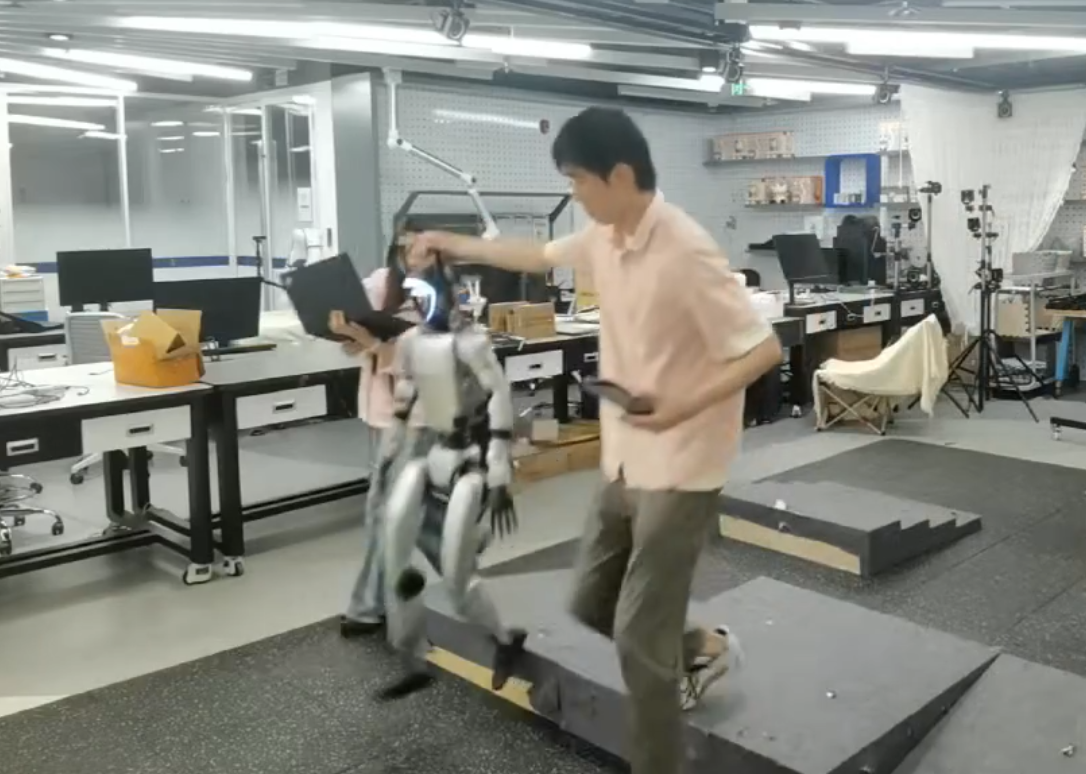
\includegraphics[width=0.9\textwidth]{figures/ch7_slope_hop_landing.png}
    \caption{The robot performing a small two-foot hop at the end of the slope to transition to flat ground, a natural and energy-efficient motion emerging from the AMP-trained gait style.}
    \label{fig:slope_hop_landing}
\end{figure}

%% ============================================================
\section{Discussion}
\label{sec:real_discussion}
%% ============================================================

\subsection{Natural Motion Style}
\label{sec:natural_motion}

A notable outcome of the real-robot experiments is the naturalness of the robot's motion. The walking gait, foot placement, and body posture adjustments all appear fluid and human-like. This is attributed to the AMP discriminator (Chapter~\ref{chap:proposed_method}), which provides a style reward that encourages the policy to imitate the reference motion data, combined with the MoE architecture that allows different experts to specialize in different terrain conditions. Without AMP, the robot's gait would be functional but robotic---achieving the task without the stylistic quality that makes the motion appear natural.

\subsection{Attention, Memory, and Temporal Depth Synergy}
\label{sec:attention_memory_synergy}

The rock terrain experiment provides the clearest evidence of the three perception components working together:

\begin{enumerate}
    \item \textbf{Attention} identifies the relevant terrain feature (flat ground between rocks, the next rock surface, the slope edge).
    \item \textbf{Memory} preserves terrain context when the depth camera can no longer see the area near the feet (rocks occluding the downward view).
    \item \textbf{Temporal depth stacking} (frame subsampling) extends the effective perception horizon, allowing the robot to retain depth information from several steps ago. The policy receives 8 depth frames subsampled from a 37-frame history at 5-frame intervals, providing an effective lookback of approximately 3.6\,s.
\end{enumerate}

Without any one of these components, the robot would likely fail on the rock terrain: without attention, it would not identify the correct foothold; without memory, it would lose track of rocks near its feet once they leave the camera's view; without temporal stacking, the depth perception horizon would be too short to inform multi-step planning.

The second stair-slope run further illustrates this synergy: the robot's decision to step over the last stair rather than onto it requires (1)~attention to perceive the terrain layout, (2)~memory to retain the stair context, and (3)~temporal depth stacking to provide a longer perception horizon. The energy penalty reward then biases the policy toward the more efficient option, but only because the perception modules provide sufficient information to the policy to determine that stepping over is safe.

\subsection{Energy-Efficient Decision Making}
\label{sec:energy_efficient}

The second run on the stair-slope terrain demonstrates that the policy makes energy-efficient decisions. By stepping over the last stair rather than stepping onto it, the robot avoids an unnecessary step. This behavior is shaped by the energy penalty reward during training ($r_{\mathrm{energy}}$, weight $-5 \times 10^{-5}$, computed as the squared sum of motor power $\tau \cdot \dot{q}$ normalized by stiffness) and enabled by the combined perception of attention, memory, and temporal depth stacking, which give the robot sufficient information to determine that stepping over is safe. Similarly, the two-foot hop at the end of the slope is a natural, energy-efficient transition that emerges from the AMP-trained gait style.

%% ============================================================
\section{Limitations}
\label{sec:real_limitations}
%% ============================================================

\begin{itemize}
    \item \textbf{Safety harness interference:} The safety harness attached to the robot's shoulders occasionally applied inadvertent tension to the robot, causing unnecessary balance corrections. This is visible in the supplementary video and slightly degrades the apparent motion quality. A fully autonomous deployment without the harness would be needed to evaluate the policy's true fall-recovery capability.

    \item \textbf{Communication reliability:} Ethernet cable disconnection was a recurring issue during testing, causing communication loss and robot falls. This is a hardware infrastructure problem rather than a policy limitation, but it highlights the importance of robust communication (or fully onboard computing) for autonomous operation.

    \item \textbf{External computing dependency:} The current deployment relies on an external laptop for policy inference, which limits the robot's autonomy and introduces a communication dependency. Future work should transition to onboard computing (e.g., NVIDIA Jetson Orin NX) to enable fully autonomous operation.

    \item \textbf{Limited extreme terrain testing:} The experiments were conducted on terrain modules with a maximum height of 20\,cm. The policy's performance on more extreme terrain (higher steps, steeper slopes, larger gaps) remains to be evaluated.

    \item \textbf{Velocity command sensitivity:} When the operator sends overly aggressive velocity commands (maximum speed via the wireless controller), the resulting motion amplitudes can exceed the policy's stable operating regime. Tuning a better command limiter would enhance robustness.
\end{itemize}